
\section{Black box inference}
\label{sec:bbi}

We derive an algorithm for black box inference over a wide
class of generative models.

\subsection{Variational objective}
\label{sec:bbi:model}

\begin{figure}[tb]
  \centering
  \begin{tikzpicture}
  \pgfmathsetseed{3}
  \node at (0,0) {
    \begin{tikzpicture}[thick]
    \draw plot [smooth cycle, samples=8,domain={1:8}] (\x*360/8+5*rnd:0.5cm+1.5cm*rnd) node at (0,0) {$\mathcal{R}$};
    \end{tikzpicture}
  };
  %\path[->,thick] (1.75,0) edge [bend left] node[above,yshift=0.125cm] {$\alpha$-inference} (3.25,0);
  \path[->,thick] (1.75,0) edge [bend left] node[above,align=center,yshift=0.125cm] {auxiliary\\inference} (3.25,0);
  \pgfmathsetseed{11}
  \node at (5,0) {
    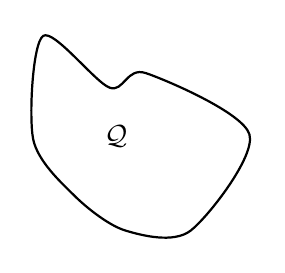
\begin{tikzpicture}[thick]
    \draw plot [smooth cycle, samples=8,domain={1:8}] (\x*360/8+5*rnd:0.5cm+1.5cm*rnd) node at (0,0) {$\mathcal{Q}$};
    \end{tikzpicture}
  };
  \path[->,thick] (6.75,0) edge [bend left] node[above,align=center,yshift=0.125cm] {variational\\inference} (8.25,0);
  \pgfmathsetseed{9}
  \node at (10,0) {
    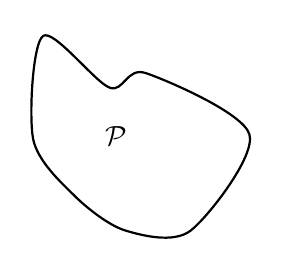
\begin{tikzpicture}[thick]
    \draw plot [smooth cycle, samples=8,domain={1:8}] (\x*360/8+5*rnd:0.5cm+1.5cm*rnd) node at (0,0) {$\mathcal{P}$};
    \end{tikzpicture}
  };
\end{tikzpicture}

\caption{Sequence of domain mappings during inference, from
variational latent variable space $\mathcal{R}$ to posterior latent
variable space $\mathcal{Q}$ to data space $\mathcal{P}$. We perform
variational inference in the posterior space and auxiliary
inference in the variational space.}
\label{fig:mappings}
\end{figure}

The original \gls{ELBO} (\myeqp{bound_autoencoder}) is
analytically intractable due to the log density,
$\log \qvgp(\mbz)$ (\myeqp{vgp}). To address this, we present a tractable variational
objective inspired by auto-encoders~\citep{kingma2014autoencoding}.

A tractable lower bound to the model
evidence $\log p(\mbx)$ can be derived by subtracting an expected KL
divergence term from the \glsunset{ELBO}\gls{ELBO},
\begin{equation*}
\log p(\mbx)
\ge
\mathbb{E}_{\qvgp}[\log p(\mbx\g\mbz)]
- \operatorname{KL}(\qvgp(\mbz)\|p(\mbz))
- \mathbb{E}_{\qvgp}\Big[
\operatorname{KL}(q(\mbxi,f\g\mbz)\|r(\mbxi,f\g\mbz))
\Big],
\end{equation*}
where $r(\mbxi,f\g\mbz)$ is an auxiliary model (we describe $r$ in
the next subsection).
Various versions of this objective have been considered in the
literature~\citep{jaakola1998improving,agakov2004auxiliary}, and it
has been recently revisited by \citet{salimans2015markov} and
\citet{ranganath2015hierarchical}.
We perform variational inference
in the posterior latent variable space, minimizing
$\operatorname{KL}(q\|p)$ to learn the variational
model; for this to occur we perform auxiliary inference in the
variational latent variable space, minimizing
$\operatorname{KL}(q\|r)$ to learn an auxiliary model.
See \myfig{mappings}.

Unlike previous approaches, we rewrite this variational objective to
connect to auto-encoders:
\begin{align}
\label{eq:variational_objective}
\begin{split}
\widetilde{\cL}(\mbtheta,\mbphi)
&
=
\mathbb{E}_{\qvgp}[\log p(\mbx\mid\mbz)]
-
\mathbb{E}_{\qvgp}\Big[
\operatorname{KL}(q(\mbz\g f(\mbxi))\|p(\mbz))
\Big]
\\
&
\quad
-
\mathbb{E}_{\qvgp}\Big[
\operatorname{KL}(q(f\g\mbxi;\mbtheta)\|r(f\g\mbxi,\mbz;\mbphi))
+
\log q(\mbxi) - \log r(\mbxi\g\mbz)
\Big],
\end{split}
\end{align}
where the KL divergences are now taken over tractable distributions
(see \myappendix{variational}).
In auto-encoder parlance, we maximize the expected negative
reconstruction error, regularized by two terms: an expected divergence between
the variational model and the original model's prior, and an expected
divergence between the auxiliary model and the variational model's
prior. This is simply a nested instantiation of the variational
auto-encoder bound~\citep{kingma2014autoencoding}: a
divergence between the inference model and a prior is taken as
regularizers on both the posterior and variational spaces. This
interpretation justifies the previously proposed
bound for variational models;
as we shall see, it also enables lower variance gradients during
stochastic optimization.

\subsection{Auto-encoding variational models}

An inference network provide a flexible parameterization of
approximating distributions as used in Helmholtz
machines~\citep{hinton1994autoencoders}, deep Boltzmann machines~\citep{salakhutdinov2010efficient}, and variational
auto-encoders~\citep{kingma2014autoencoding,rezende2014stochastic}.
It replaces local variational parameters with global parameters
coming from a neural network. For latent variables $\mbz_n$
(which correspond to a data point $\mbx_n$), an inference network
specifies a neural network which takes $\mbx_n$ as input and its local
variational parameters $\mblambda_n$ as output.  This amortizes
inference by only defining a set of global parameters.


To auto-encode the \gls{VGP} we specify inference networks to
parameterize both the variational and auxiliary models:
\begin{equation*}
\mbx_n\mapsto q(\mbz_n\g\mbx_n; \mbtheta_n),
\qquad
\mbx_n,\mbz_n\mapsto r(\mbxi_n,f_n\g\mbx_n,\mbz_n;
\mbphi_n).
\end{equation*}
Formally, the output of these mappings are the parameters $\mbtheta_n$ and
$\mbphi_n$ respectively. We write the output as distributions above to emphasize
that these mappings are a (global) parameterization of the variational
model $q$ and auxiliary model $r$.
The local variational parameters $\mbtheta_n$ for $q$ are the
variational data $\cD_n$. The auxiliary model $r$ is specified as a fully factorized
Gaussian with local variational parameters
$\mbphi_n=(\mbmu_n\in\mathbb{R}^{c+d}$,
$\mbsigma^2_n\in\mathbb{R}^{c+d})$.  \footnote{We let the kernel
hyperparameters of the \gls{VGP} be fixed across data points.
Note also that unique from other auto-encoder approaches, we let $r$'s
inference network take both $\mbx_n$ and $\mbz_n$ as input: this
avoids an explicit specification of the conditional distribution
$r(\mbepsilon,f\g\mbz)$, which may be difficult to model.
This idea was first suggested (but not implemented) in
\citet{ranganath2015hierarchical}.
}

\subsection{Stochastic optimization}
\label{sec:bbi:gradient}

We maximize the variational objective
$\widetilde{\cL}(\mbtheta,\mbphi)$ over both $\mbtheta$ and $\mbphi$, where
$\mbtheta$ newly denotes both the kernel hyperparameters and
the inference network's parameters for the \gls{VGP}, and $\mbphi$
denotes the
inference network's parameters for the auxiliary model.
Following black box methods, we write
the gradient as an expectation and apply stochastic
approximations~\citep{robbins1951stochastic}, sampling from the
variational model and evaluating noisy gradients.

First, we reduce variance of the stochastic gradients by analytically
deriving any tractable expectations.
The KL divergence between
$q(\mbz\g f(\mbxi))$ and $p(\mbz)$ is commonly used to reduce
variance in traditional variational auto-encoders: it is analytic for
deep generative models such as the deep latent Gaussian
model~\citep{rezende2014stochastic} and deep recurrent
attentive writer~\citep{gregor2015draw}.
The KL divergence between
$r(f\g\mbxi,\mbz)$ and $q(f\g\mbxi)$ is analytic as the distributions
are both Gaussian. The difference $\log q(\mbxi) - \log
r(\mbxi\g\mbz)$ is simply a difference of Gaussian log densities.
See \myappendix{variational} for more details.

To derive black box gradients, we can first reparameterize the
\gls{VGP}, separating noise generation of samples from
the parameters in its generative
process~\citep{kingma2014autoencoding,rezende2014stochastic}. The
\gls{GP} easily enables reparameterization:
for latent inputs $\mbxi\sim\mathcal{N}(\mbzero,\mbI)$,
the transformation
$\f(\mbxi;\mbtheta)=\mbL\mbxi + \Kxis \Kss^{-1} \mbt_i$
is a location-scale transform,
where $\mbL\mbL^\top = \Kxixi - \Kxis \Kss^{-1} \Kxis^\top$.
This is equivalent to evaluating $\mbxi$ with a random mapping
from the \gls{GP}.
Suppose the mean-field $q(\mbz\g f(\mbxi))$ is also reparameterizable,
and let $\mbepsilon\sim w$ such that $\mbz(\mbepsilon;\f)$ is a
function of $\mbepsilon$ whose output $\mbz\sim q(\mbz\g f(\mbxi))$.
This two-level reparameterization is equivalent to the generative
process for $\mbz$ outlined in \mysec{vgp}.


We now rewrite the variational objective as
\begin{align}
\label{eq:reparam_objective}
\widetilde{\cL}(\mbtheta,\mbphi)
&
=
\mathbb{E}_{\mathcal{N}(\mbxi)}\Big[\mathbb{E}_{w(\mbepsilon)}\Big[
\log p(\mbx\mid\mbz(\mbepsilon;\f))
\Big]
-
\operatorname{KL}(q(\mbz\g \f)\|p(\mbz))
\Big]
\\
&
\quad
-
\mathbb{E}_{\mathcal{N}(\mbxi)}\Big[\mathbb{E}_{w(\mbepsilon)}\Big[
\operatorname{KL}(q(f\g\mbxi;\mbtheta)\|r(f\g\mbxi,\mbz(\mbepsilon;\f);\mbphi))
+
\log q(\mbxi) - \log r(\mbxi\g\mbz(\mbepsilon;\f))
\Big]\Big].
\nonumber
\end{align}
\myeqp{reparam_objective} enables gradients to move inside the expectations and backpropagate over
the nested reparameterization. Thus we can take unbiased stochastic
gradients, which exhibit low variance due to both the analytic
KL terms and reparameterization.
The gradients are derived in
\myappendix{gradients}, including the case when the first KL is
analytically intractable.

\begin{algorithm}[t]
  \caption{Black box inference with a \acrlong{VGP}}
  \SetAlgoLined
  \DontPrintSemicolon
  \BlankLine
  \KwIn{Model $p(\mbx,\mbz)$, Mean-field family $\prod_i q(\mbz_i\g
  f_i(\mbxi))$.}
  \BlankLine
  \textbf{Output}: Variational and auxiliary parameters
  $(\mbtheta,\mbphi)$.\;
  \BlankLine
  Initialize $(\mbtheta,\mbphi)$ randomly.
  \BlankLine
  \While{\textnormal{not converged}}{
    \BlankLine
    Draw noise samples $\mbxi\sim\mathcal{N}(\mbzero,\mbI)$,
    $\mbepsilon\sim w$.\;
    \BlankLine
    Parameterize variational samples
    $\mbz = \mbz(\mbepsilon;f(\mbxi))$, $f(\mbxi)=\f(\mbxi;\mbtheta)$.
    \BlankLine
    Update $(\mbtheta,\mbphi)$ with stochastic gradients
    $\nabla_{\mbtheta}\widetilde{\cL}$,
    $\nabla_{\mbphi}\widetilde{\cL}$.
  }
  \label{alg:vgp}
\end{algorithm}

We outline the method in \myalg{vgp}. For massive data, we
apply subsampling on
$\mbx$~\citep{hoffman2013stochastic}. For gradients of the model
log-likelihood, we employ convenient differentiation tools such as
those in Stan and Theano~\citep{carpenter2015stan,bergstra2010theano}.
For non-differentiable latent variables $\mbz$, or mean-field
distributions without efficient reparameterizations,
we apply the black box gradient estimator from \citet{ranganath2014black} to take gradients of the inner expectation.

\subsection{Computational and storage complexity}

The algorithm
has $\mathcal{O}(d+m^3+LH^2)$ complexity, where $d$ is the number of
latent variables, $m$ is the size of the variational data, and $L$
is the number of layers of the neural networks with $H$ the average
hidden layer size.
In particular, the algorithm is linear in the number of latent
variables, which is competitive with other variational inference methods.
The number of variational and auxiliary parameters has
$\mathcal{O}(c+LH)$ complexity; this complexity comes from storing the kernel
hyperparameters and the neural network parameters.
\if0
Note that unlike most literature applying \glspl{GP}, we require no
low rank constraints such as the use of inducing
variables~\citep{quinonero2005unifying}.
or
subsampling of the variational data~\citep{hensman2013gaussian}.
Such constraints are typically employed to reduce the high cost of
\gls{GP} inference, cubic in the size of the regressed data set.  In
the \gls{VGP} setting, the size $m$ of the variational data (along
with its input and output locations) is already subject to our
control.
\PP
The size of the variational data linearly scales the number of outputs
for the inference networks, which may be too large for an inference
network to learn for moderate size data in practice.
See \myappendix{size} for details on scaling to massive sizes of
variational data if necessary.
\fi

Unlike most \gls{GP} literature, we require no low rank constraints,
such as the use of inducing variables
for scalable computation~\citep{quinonero2005unifying}. The variational data serve a similar
purpose,
but inducing variables reduce the rank of a (fixed) kernel matrix; the
variational data directly determine the kernel matrix and thus the
kernel matrix is not fixed.
Although we haven't found it necessary in practice, see
\myappendix{size} for scaling the size of variational data.

